\documentclass[12pt,a4paper]{article}

\usepackage{graphicx}                            % Para poder incluir gráficos.
\usepackage[brazilian]{babel}                    % Para separar as sílabas, e colocar os nomes padrão (capítulo, bibliografia, etc.) em português.
\usepackage[utf8]{inputenc}                      % Para poder escrever diretamente com acentos, sem ter que usar códigos.
\usepackage[T1]{fontenc}                         % Para poder copiar do PDF acentos.
\usepackage{natbib}                              % \citep{jon90} --> (Jones et al., 1990)
\usepackage[colorlinks,citecolor=blue]{hyperref} % Para colocar links nas referências, equações, figuras, etc, além de menu árvore no PDF.
\usepackage{verbatim}                            % Para poder comentar regiões do arquivo .tex 
\usepackage[small,bf]{caption}                   % Para que legendas de figuras e tabelas fique em fonte menor e com negrito.
\usepackage{amssymb}                             % Para poder utilizar alguns símbolos matemáticos especiais.
\usepackage{amsmath}                             % Para poder usar o comando 'cases', e possivelmente outros.
\usepackage{fancyhdr}                            % Para poder fazer cabeçalhos e rodapés mais bonitos.
%\usepackage{epstopdf}                            % Para poder usar imagens .eps no compilador pdflatex (que permite usar imagens .png).
\usepackage{times}                               % Para usar typeset bem definido.
\usepackage{titlesec}                            % Para poder redefinir o formato dos títulos de seções

\usepackage[svgnames]{xcolor}                              
\usepackage{helvet}
\usepackage{lipsum}


%%% Formatting %%%
\definecolor{MSBlue}{rgb}{.204,.353,.541}
\definecolor{MSLightBlue}{rgb}{.31,.506,.741}
\newcommand{\secColor}{\color{RoyalBlue}}
\setlength\headheight{26pt} %% just to make warning go away. Adjust the value after looking into the warning.
\titleformat*{\section}{\LARGE\bfseries\sffamily\secColor}
\titleformat*{\subsection}{\Large\bfseries\sffamily\secColor}
\titleformat*{\subsubsection}{\normalsize\bfseries\sffamily\secColor}
\renewcommand{\headrule}{\secColor\hrule}

%%% Commands %%%
\newcommand{\myurl}[1]{{\footnotesize\url{#1}}}

\pagestyle{fancy}
\author{Henrique S. Xavier \& João Carabetta}
\title{\Huge\sffamily\bfseries 100 dias de congresso}

% \rhead{{\color{blue}\rule{1cm}{1cm}}}

\fancyhead[L]{\fontsize{10}{12}\sffamily\secColor\rightmark}
\rhead{
\includegraphics[width=3cm]{acredito_fundobranco.png}}


%%%%%%%%%%%%%%%% REPORT %%%%%%%%%%%%%%%%%%
\begin{document}
\pagenumbering{gobble}
\thispagestyle{empty}
\maketitle
%\tableofcontents

\pagebreak
\thispagestyle{plain}
\pagenumbering{arabic}
\section{Introdução}
\label{sec:intro}

Este trabalho visa apresentar um panorama do congresso nacional brasileiro nos 100 primeiros dias da $56^{\mathrm{\underline{a}}}$ legislatura, que
se iniciou no dia 1 de fevereiro de 2019, utilizando as bases de dados abertos da câmara\footnote{\myurl{http://dadosabertos.camara.leg.br/}}
e do senado\footnote{\myurl{http://www12.senado.leg.br/dados-abertos}}. Além de apresentar o cenário atual, também buscamos analisar
as características históricas do congresso, tanto para fins de comparação quanto de construção de um retrato de suas características
mais estruturais. Os objetivos deste relatório são dois: de servir de subsídio para a atividade parlamentar do movimento Acredito na
câmara e no senado, e de prover à sociedade mais informações relativas ao trabalho de seus representantes e das estruturas governamentais
utilizadas nessa representação.

Dado o curto período de tempo disponível para a realização deste estudo, apresentamos aqui uma análise inicial que
certamente poderá ser desdobrada e aprofundada em investigações futuras. Essa análise foi segmentada em duas frentes,
uma focada nos parlamentares e outra nas proposições -- e.g. projetos de lei (PLs), medidas provisórias (MPs) e propostas
de emendas à constituição (PECs) -- em tramitação.

Em relação aos parlamentares, buscamos investigar:
(\emph{i}) o uso da cota parlamentar (verba destinada a cobrir os custos do trabalho parlamentar);
(\emph{ii}) o apoio ao governo e a fidelidade partidária;
(\emph{iii}) a distribuição de cargos e poder;
(\emph{iv}) e o nível de participação e engajamento.
Em relação às proposições, analisamos quais temas são os mais recorrentes historicamente e na atual legislatura.

Um de nossos primeiros achados se refere à limitação das bases de dados, particularmente em relação
aos dados mais recentes. Por exemplo, os parlamentares tem um prazo de 90 dias para solicitar reembolso
à cota parlamentar\footnote{\myurl{https://www2.camara.leg.br/comunicacao/assessoria-de-imprensa/cota-parlamentar}}
e empresas aéreas chegam a demorar mais do que isso para comunicar à câmara a emissão de
bilhetes, o que torna incompleta a amostra de gastos dos últimos 100 dias. Nesses casos, optamos por apenas
realizar uma análise histórica.

\section{Parlamentares}

\subsection{Uso da cota parlamentar}

Conforme apresentado na Seção \ref{sec:intro}, as bases de dados relacionadas às despesas parlamentares dos 100 últimos
dias ainda estão sendo atualizadas. As referentes ao ano de 2018 ganharam, em média, 530 entradas por dia desde o início
dessa análise, em grande parte relativas à emissão de bilhetes aéreos. Essa incompleteza da base de dados se evidencia
na Fig. \ref{fig:n-despesas-por-mes}. A queda abrupta, a partir de 2018, no número de despesas registradas é ao menos
em parte consequência dessa defasagem no registro dos gastos. A Fig. \ref{fig:n-despesas-por-mes} ainda mostra que
os gastos do total de deputados segue um padrão recorrente ao longo dos anos, com uma queda significativa em janeiro.

\begin{figure}[t]
\centering
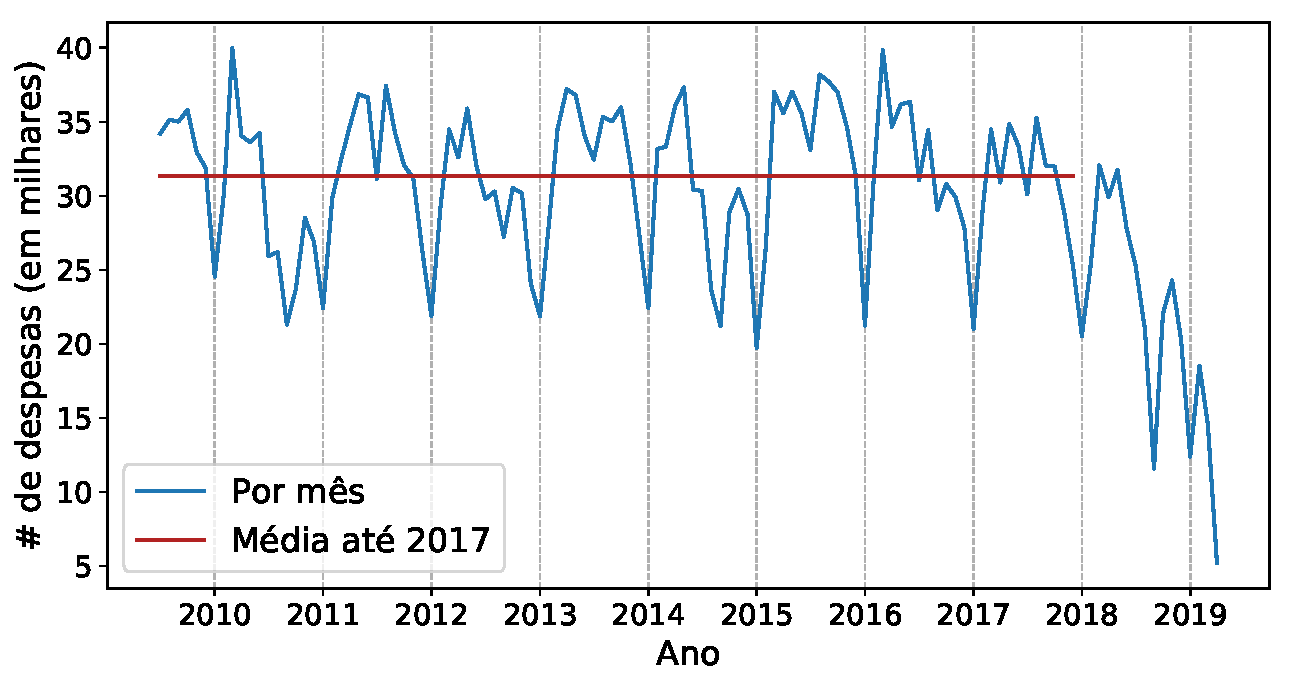
\includegraphics[width=1.0\textwidth]{graficos/n_despesas_por_mes_2019-04-29.pdf}
\caption{Número de despesas na base de dados de uso da cota parlamentar dos deputados federais
  referentes a cada mês, em função do tempo (em azul).
  A linha vermelha indica o número médio de 2009 a 2018.}
\label{fig:n-despesas-por-mes}
\end{figure} 

Para acompanhar o valor total gasto com a cota parlamentar ao longo do tempo, nós primeiro deflacionamos os
valores pelo IPCA e em seguida o decompusemos num modelo aditivo com termos de tendência geral, sazonalidade e
resíduo (veja a Fig. \ref{fig:total-despesas-por-mes}). Através da curva de tendência, podemos notar que
o valor médio gasto praticamente não se alterou desde 2010, sendo que uma leve queda pode ser notada em anos
recentes. Ressaltamos que ao menos parte dessa queda é consequência da defasagem de registro dos gastos.

\begin{figure}[t]
\centering
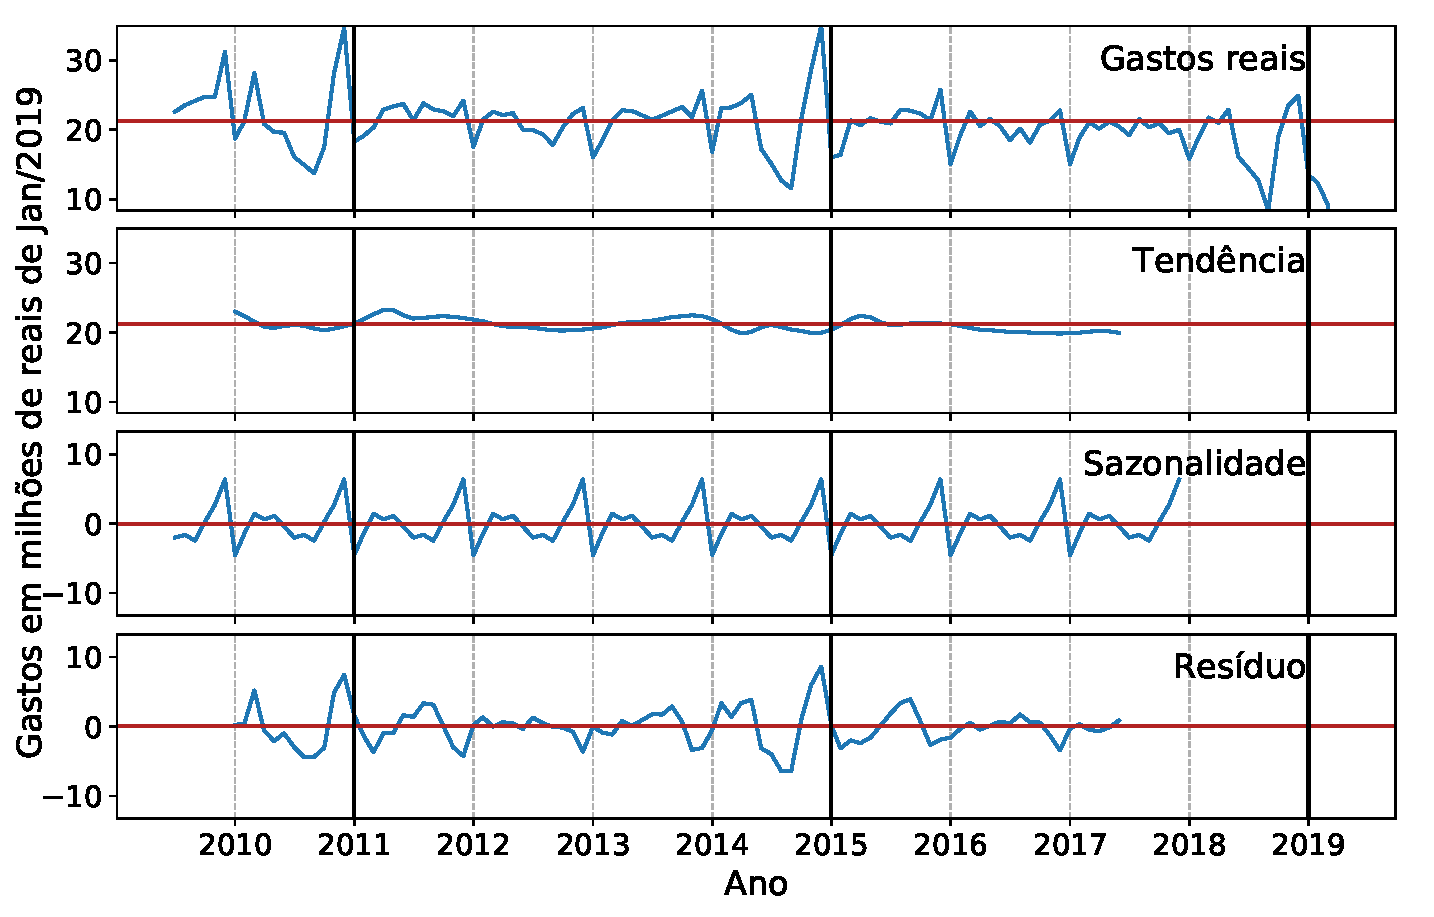
\includegraphics[width=1.0\textwidth]{graficos/despesas-reais-e-sazonalidade_2019-04-29.pdf}
\caption{Valor real (descontada a inflação) gasto com o exercício da atividade parlamentar em cada mês
  (reembolsos feitos dentro da cota parlamentar, em azul). O painel superior mostra o valor observado, e os
  abaixo mostram as contribuições de: tendência geral, calculada através de uma média móvel; sazonalidade; e resíduo.
  A linha vermelha indica o valor médio em todo o período (nos dois painéis superiores) e o zero (nos dois
  painéis inferiores). A decomposição em contribuições aditivas foi feita até o ano de 2017.}
\label{fig:total-despesas-por-mes}
\end{figure} 

Também é possível notar que os gastos apresentam uma sazonalidade bastante marcada, com quedas mais
acentuadas em janeiro e picos em dezembro. Esses picos podem decorrer do fato de que a cota parlamentar, mensal,
pode ser acumulada ao longo do ano mas não pode ser transferida para o exercício financeiro seguinte.
É possível percebem ainda, tanto nos gráficos do valor observado quanto no de resíduos, que existe
um pico ainda mais acentuado ao final de cada legislatura (marcadas com linhas verticais pretas contínuas).
Esse pico parece ser precedido por uma queda nos gastos, possivelmente indicando uma estratégia de acúmulo de verba
para a realização de um último gasto em dezembro.

Por fim, verificamos como o valor total reembolsado pela cota parlamentar se divide nas categorias pré-definidas
pela câmara. A Figura \ref{fig:despesas-por-tipo} mostra a fração do valor total que é destinada a cada categoria
de gastos. Verificamos que os maiores gastos realizados são com divulgação da atividade parlamentar (que, em geral,
apresentam valores altos para uma única despesa e perfazem 20\% do total) e com transporte aéreo: somando as rubricas
``emissão de bilhere aéreo'', ``locação ou fretamento de aeronaves'' e ``passagens aéreas'', temos cerca de
23\% dos gastos. Em grande medida, esse montante deriva do deslocamento semanal do deputado ao seu estado de origem.
Gastos com manutenção de escritório de apoio em seu estado, consultorias, telefonia e transportes terrestres vêm
em seguida. Junto com passagens aéreas, o transporte totaliza cerca de 44\% do total. Gastos com alimentação e
hospedagem fora do distrito federal totalizam, em média, menos de 2\% dos gastos.



\begin{figure}[t]
\centering
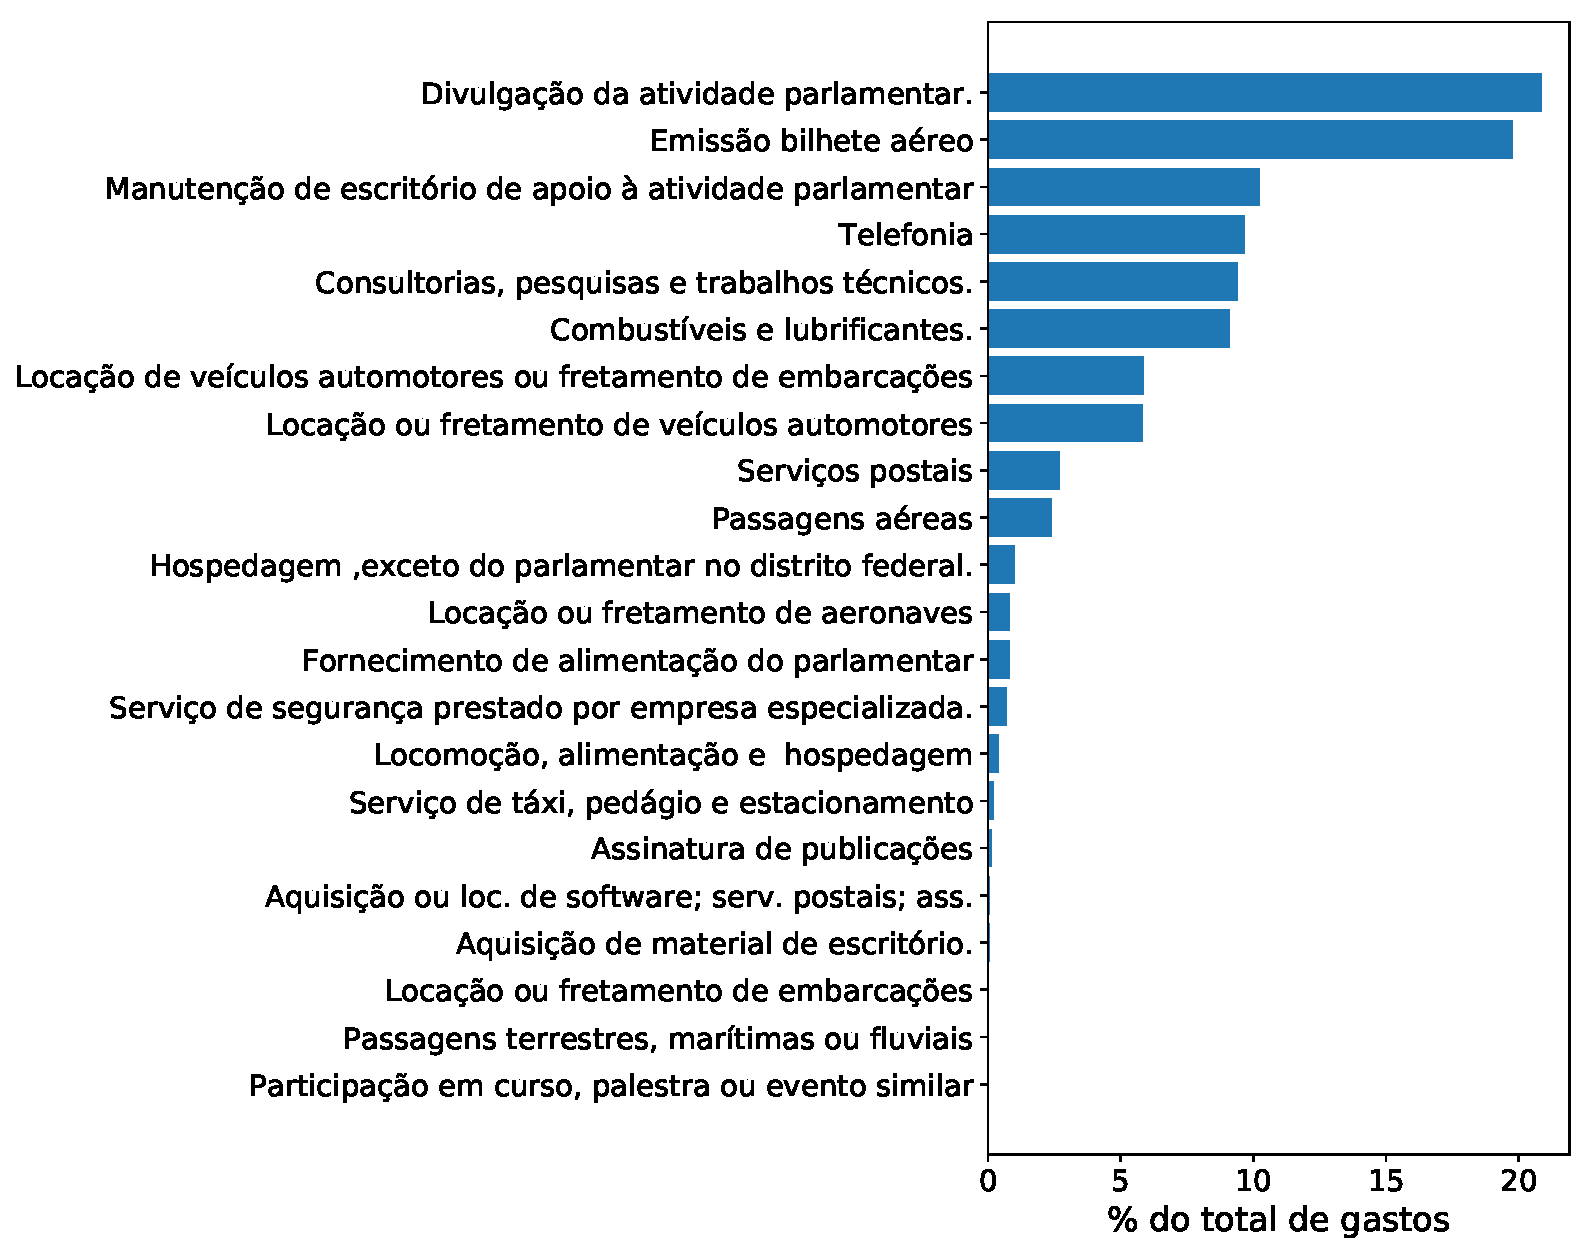
\includegraphics[width=1.0\textwidth]{graficos/total-despesas-por-tipo_2019-04-29.pdf}
\caption{Porcentagem do valor total utilizado pelos deputados federais que é destinado a cada finalidade. Nesse
cálculo, utilizamos os valores de 2009 a 2017, corrigigos pela inflação.}
\label{fig:despesas-por-tipo}
\end{figure} 


\subsection{Análise das votações}
\subsection{Distribuição de cargos e poder}
\subsection{Atividade parlamentar}


\section{Proposições}

\end{document}
